\documentclass[onlymath, nologo]{beamer}

\usepackage{amsmath, amsfonts}
\usepackage{tikz}
\usepackage{tabulary}
\usepackage{array}
{\renewcommand{\arraystretch}{2}%
\usepackage{mathtools}
\setbeamertemplate{caption}{\raggedright\insertcaption\par}
\usepackage{multimedia}
\usepackage[version=4]{mhchem}
\usepackage[theorems, skins]{tcolorbox}

\graphicspath{{../figs/}}

\definecolor{UTBlue}{RGB}{94,156,174}
\definecolor{HCrimson}{RGB}{165,28,48}
\definecolor{HInk}{RGB}{30,30,30}
\definecolor{HMortar}{RGB}{140,129,121}
\definecolor{HParchment}{RGB}{243,243,241}
\definecolor{HSlate}{RGB}{137,150,160}
\definecolor{HShade}{RGB}{186,197,198}
\tcbset{colback=HParchment,colframe=HCrimson}

\usetheme[white]{Harvard}

\author[]{Instructor:  David Sondak \\ TFs:  Charles Liu, Eric Wu and Kevin Wu}
\title{CS207: Systems Development for Computational Science}
\subtitle{\url{https://iacs-cs-207.github.io/cs207-F17/}}

\institute{Harvard University \\ 
           Institute for Applied Computational Science}
\date{\large 8/30/2017}

\begin{document}

\bgroup
\makeatletter
\setbeamertemplate{footline}{}
\makeatother

  \begin{frame}
    \titlepage
  \end{frame}
  \egroup
  
  \setcounter{framenumber}{0}

  \begin{frame}{Motivation:  Thermal Convection and the Geodynamo}
    \uncover<1->{
        {\centering \textbf{\textcolor{HCrimson}{Thermal convection drives most fluid flows in the universe}} \\[0.5em]}
    }
    \uncover<2->{
    \begin{columns}[T]
      \begin{column}{0.6\textwidth}
        \uncover<2->{
        \centering
        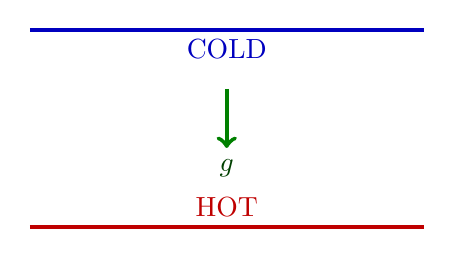
\begin{tikzpicture}
          \draw[ultra thick, blue!75!black] (0,2.5) -- (5,2.5);
          \draw[ultra thick, red!75!black]  (0,0) -- (5,0);
          \draw (2.5,2.5) node [blue!75!black, below] {COLD};
          \draw (2.5,0.0) node [red!75!black, above] {HOT};
          \draw[ultra thick, green!50!black, ->] (2.5, 1.75) -- (2.5, 1.0) node [below] {$\textcolor{green!25!black}{g}$};
        \end{tikzpicture}
        \\[1.0em]
        Cold fluid falls, hot fluid rises \\[0.5em]
        \href{https://www.youtube.com/watch?v=ryrXAGY1dmE}{\beamergotobutton{Plate Tectonics Video}}
        }
      \end{column}
      \begin{column}{0.4\textwidth}
        \uncover<3->{
        \centering
        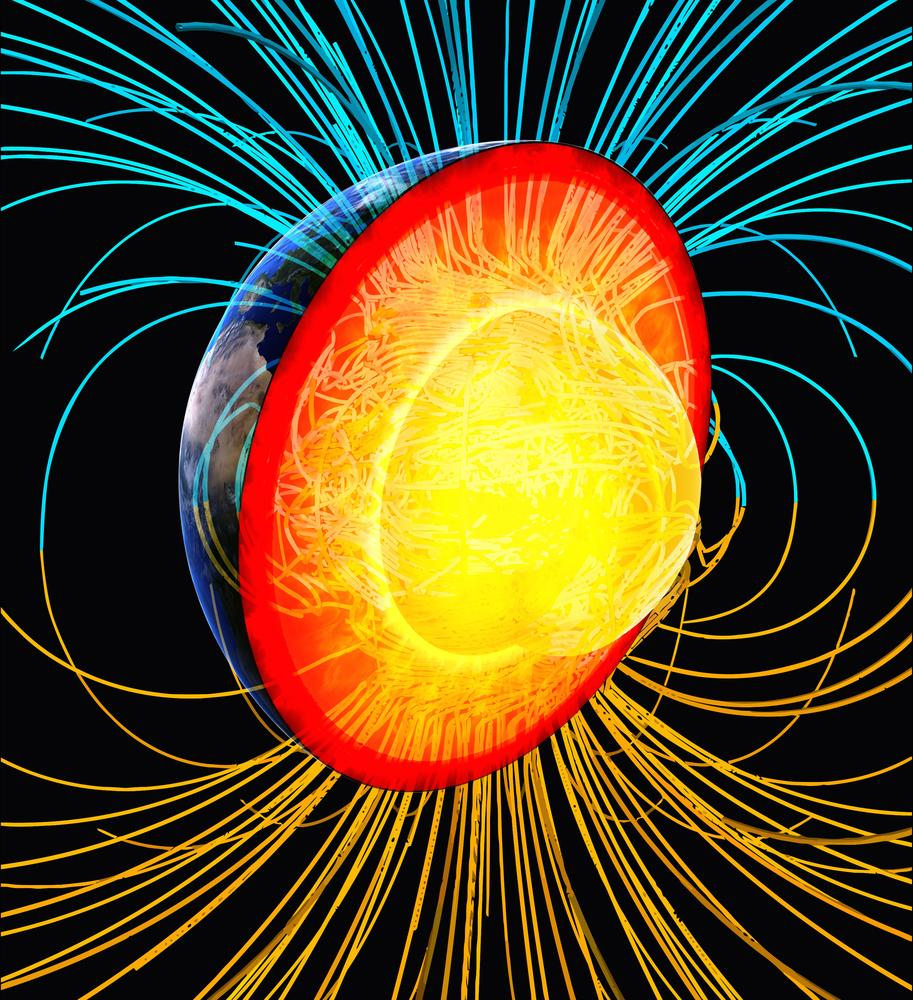
\includegraphics[width=0.75\textwidth]{geodynamo.jpg} \\[-0.1em]
        {\tiny \href{http://www.desy.de/news/news_search/index_eng.html?openDirectAnchor=1047}{DESY}}
        }
      \end{column}
    \end{columns}
    \vspace{-0.25em}
    }
    \uncover<4->{
    \begin{align*}
      \tcboxmath{\frac{\partial T}{\partial \mathrm{t}} + \nabla\cdot\left(\mathbf{u}T\right) = k\nabla^{2}T} %\quad 
      %\tag*{\movie[externalviewer]{\textcolor{blue!75!black}{\small \textbf{Convection Movie}}}{TC.ogv}}
    \end{align*}
    \vspace{-0.25em}
    \begin{itemize}
      \item Ignoring $\displaystyle \nabla\cdot\left(\mathbf{u}T\right)$ gives the usual heat conduction equation! %\\[0.5em]
      %\item In general, the full equation is impossible to solve analytically
    \end{itemize}
    }
  \end{frame}

  \begin{frame}{Motivation:  The Pillars of Science}
    \centering
    \includegraphics<1>[width=0.65\textwidth]{old_pillars.pdf}
    \includegraphics<2>[width=0.65\textwidth]{new_pillars.pdf}
  \end{frame}

  \begin{frame}{Computational Science}
    \vspace{-0.8em}
    \begin{center}
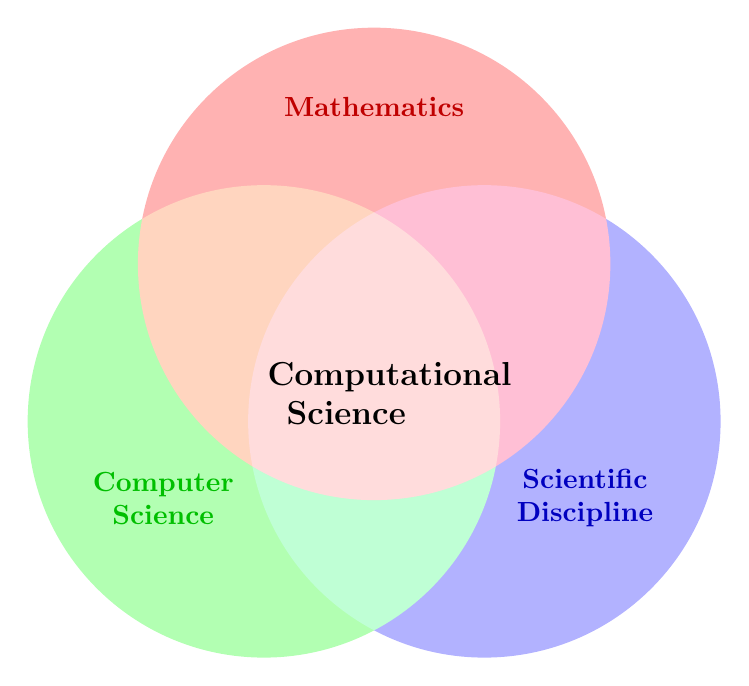
\begin{tikzpicture}
  \begin{scope}[blend group = soft light]
    %\fill[red!30!white]   ( 90:2.0) circle (3);
    %\fill[green!30!white] (160:2.0) circle (3);
    %\fill[blue!30!white]  (20:2.0) circle (3);
    \fill[red!30!white]   ( 90:2.0) circle (3);
    \fill[green!30!white] (180:1.4) circle (3);
    \fill[blue!30!white]  (360:1.4) circle (3);
  \end{scope}
  \node at ( 90:4)    {\textcolor{red!75!black}{\textbf{Mathematics}}};
  \node [text centered, text width = 2cm] at (200:2.85)   {\textcolor{green!75!black}{\textbf{Computer Science}}};
  \node [text centered, text width = 2cm] at (340:2.85)   {\textcolor{blue!75!black}{\textbf{Scientific Discipline}}};
  \node [font=\large, text centered, text width = 2cm] at (135:0.5) {\textbf{Computational Science}};
\end{tikzpicture}
\end{center}

  \end{frame}

  \begin{frame}{Why take this class?}
    \begin{columns}[T]
      \begin{column}{0.7\textwidth}
        \begin{itemize}
          \item Scientific software is complex 
          \item Your code needs to be:
            \begin{itemize}
              \item Reuseable 
              \item Portable 
              \item Robust
            \end{itemize}
          \item Must go beyond ``scripting'' \\[1.0em]
        \end{itemize}
        \vfill
        \uncover<3->{
        \begin{tcolorbox}[title=CS207 Objectives, arc is angular]
            \centering
            To give students who may not have a 
            traditional computer science background the knowledge 
            and tools to develop and maintain effective software 
            for computational science applications.
        \end{tcolorbox}
        }
      \end{column}
      \begin{column}{0.3\textwidth}
        \includegraphics<2->[width=\textwidth]{frustrated_coder.jpg} \hfill \\[1.0em]
        \includegraphics<4->[width=\textwidth]{happy_coder.jpg}
      \end{column}
    \end{columns}
  \end{frame}

  \begin{frame}{Who should take this class?}
    \begin{itemize}
      \item Any kind of scientist is welcome to take this class! \\[1.0em]
      \item This course is computer science for people who aren't computer scientists:
      \begin{itemize}
        \item Data scientists
        \item Biologists
        \item Chemists
        \item Engineers 
        \item Physicists
        \item Mathematicians
        \item Economists
        \item \hspace{2.0em} \vdots %\\[1.0em]
      \end{itemize}
      \item It is also for computer scientists who want to develop scientific software \\[1.0em]
      \item CS207 is for students who need to know effective and modern software practices for 
            their career
    \end{itemize}
  \end{frame}

  \begin{frame}{Sample Topics}
    \uncover<1->{
      A few selected topics to be covered:
      \begin{columns}[T]
        \begin{column}{0.5\textwidth}
          \begin{itemize}
            \item Version control
            \item Python (basics)
            \item How Python works
            \item Software documentation
          \end{itemize}
        \end{column}
        \begin{column}{0.5\textwidth}
          \begin{itemize}
            \item Software testing
            \item Object-oriented programming
            \item Data structures
            \item Databases
          \end{itemize}
        \end{column}
      \end{columns}
      \vfill
    }
    \uncover<2->{
      \begin{columns}[b]
        \begin{column}{0.5\textwidth}
          Other potential topics \\ (not guaranteed):
          \begin{itemize}
            \item Debuggers and debugging
            \item Build systems (Make files, autotools, ...)
            \item Compiled languages
            \item Navigating a Unix OS
          \end{itemize}
        \end{column}
        \begin{column}{0.5\textwidth}
          \href{https://en.wikipedia.org/wiki/Software_bug}{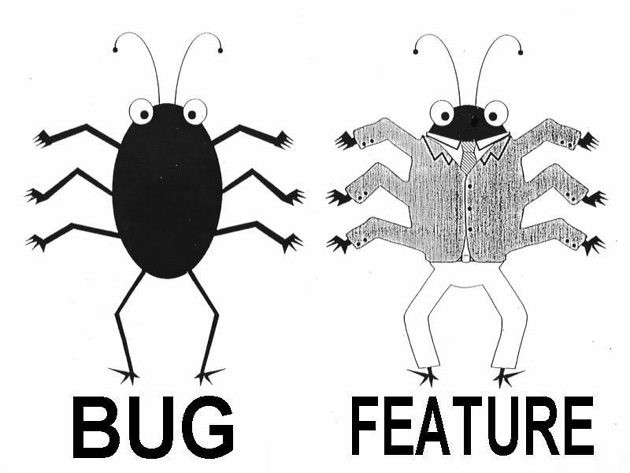
\includegraphics[width=\textwidth]{bug.jpg}}
        \end{column}
      \end{columns}
    }
  \end{frame}

  \begin{frame}{Course Structure}
    \begin{itemize}
      \item CS207 is an application-driven course \\[0.5em]
      \item Two, $1.5$ hour lectures per week \\[0.5em]
      \item Lectures centered around group programming exercises using Jupyter notebooks  \\[0.5em]
      \item ``Weekly'' programming assignments for homework \\[0.5em]
      \item Primary deliverable is a software development project \\[0.5em]
      \item All course content hosted on GitHub
    \end{itemize}
    \vfill
    \centering
    \Large Course Website:  \url{https://iacs-cs-207.github.io/cs207-F17/}
  \end{frame}

  \begin{frame}{Course Project:  Overview}
    \begin{itemize}
      \item You will work in groups of $3$ to $4$ people (assigned by teaching staff) \\[0.75em]
      \item You will add to your library throughout the semester \\[0.75em]
      \item You will demo your progress for a midterm presentation  \\[0.25em]
        \begin{itemize}
          \item Includes a proposal of your final project \\[0.75em]
        \end{itemize}
      \item For the final project, you will add a non-trivial feature to your library \\[0.75em]
      \item A portion of your grade will come from peer-assessment \\[0.75em]
      \item Exact details on website
    \end{itemize}
  \end{frame}

  \begin{frame}{Course Project:  The Topic}
    \uncover<1->{
    \begin{itemize}
      \item<1-> We will write a chemical kinetics library!
    \end{itemize}
    }
    \uncover<2->{
    \begin{columns}[c]
      \begin{column}{0.5\textwidth}
        \centering
        \uncover<2->{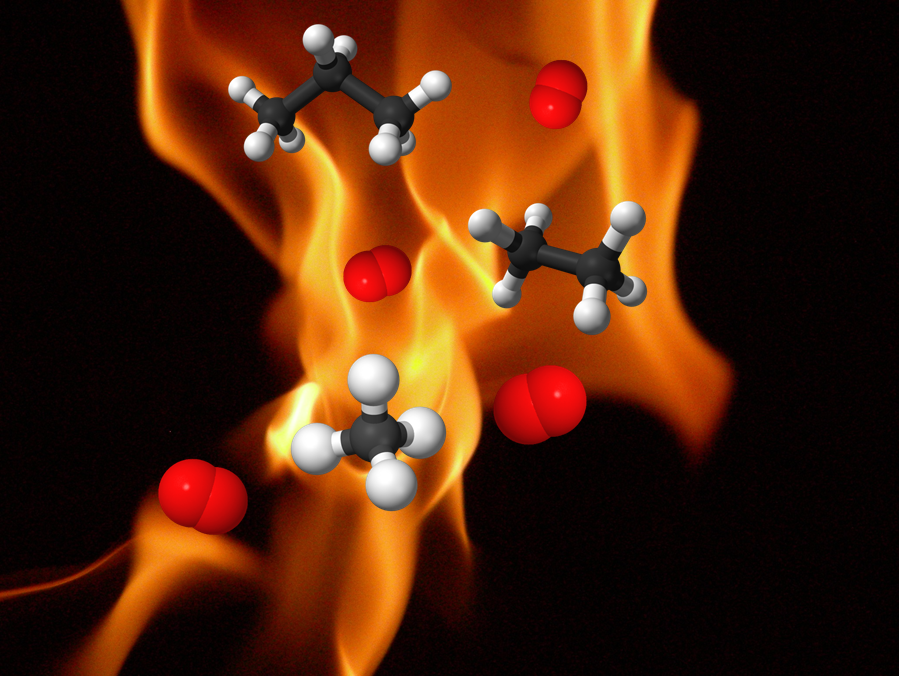
\includegraphics[width=\textwidth]{combustion.png} \hfill \\}
        \uncover<2->{\tiny Combustion Kinetics Course, Technische Universitat Berlin}
      \end{column}
      \begin{column}{0.5\textwidth}
        \centering
        \uncover<3->{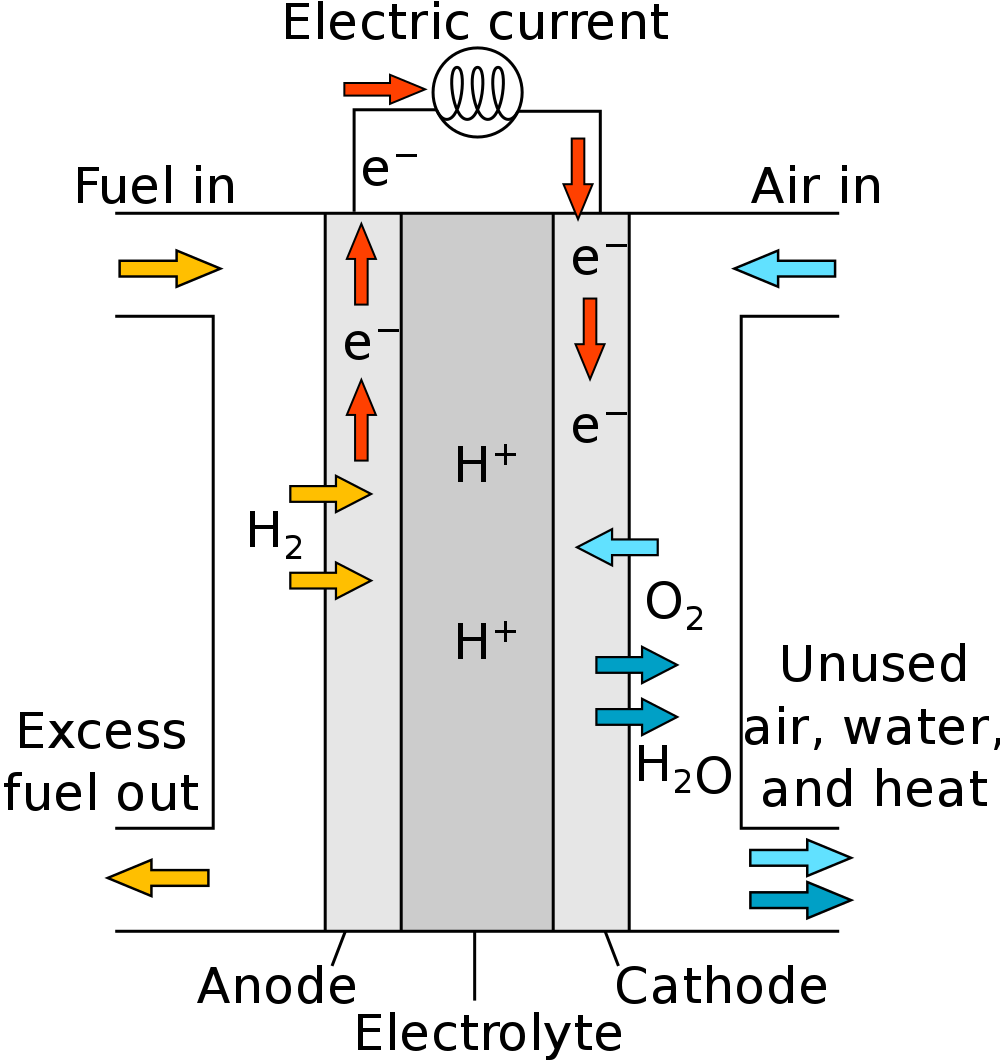
\includegraphics[width=\textwidth]{PEM_fuel_cell.png} \hfill \\}
        \uncover<3->{\tiny \url{https://commons.wikimedia.org/wiki/File:Proton_Exchange_Fuel_Cell_Diagram.svg}}
      \end{column}
    \end{columns}
    }
  \end{frame}

  \begin{frame}{Course Project:  Why Kinetics???}
    \begin{itemize}
      \item Very popular area of study \\[0.25em]
        \begin{itemize}
          \item Examples in physics, engineering, machine learning, and data science \\[1.0em]
        \end{itemize}
      \item The mathematics is accessible
      \begin{columns}{c}
        \begin{column}{0.5\textwidth}
          \begin{align*}
            \ce{H2} + \ce{O2} \ce{<=>[k1]} \ce{H2O} + \ce{O} \\
            %\ce{H} + \ce{OH} \ce{<=>} \ce{H2} + \ce{O} \\
            \ce{H2} + \ce{O2} + \ce{M} \ce{<=>[k2]} \ce{H2O2} + \ce{M} 
          \end{align*}
        \end{column}
        \begin{column}{0.5\textwidth}
          \begin{align*}
            \frac{\mathrm{d}\mathbf{x}}{\mathrm{d}t} = 
              \underbrace{\textcolor{HCrimson}{\mathbf{f}\left(\mathbf{x}\right)}}_{\textrm{return this}}
          \end{align*}
        \end{column}
      \end{columns}
      \item Good, clean, non-trivial example for illustration of software development principles \\[1.0em]
    \end{itemize}
    \begin{tcolorbox}[title=Important Note on Expectations, arc is angular]
        \centering
        You are not responsible for becoming an expert in chemical kinetics!  You will not be tested 
        on your kinetics proficiency.
    \end{tcolorbox}
  \end{frame}

  \begin{frame}{Next Steps}
    Go to \url{https://github.com/IACS-CS-207/cs207-F17/blob/master/lectures/L1/L1.ipynb}.
  \end{frame}

  \begin{frame}{Set up GitHub and get the course repository}
    \begin{itemize}
      \item If you don't already have a GitHub account, go to \url{https://github.com/} and create an account. 
      \item From your GitHub homepage, find the \textcolor{green!75!black}{\textbf{New Repository}} button:
        \begin{enumerate}
          \item Click the \textcolor{green!75!black}{\textbf{New Repository}} button. 
          \item Name the repository \texttt{cs207\_firstname\_lastname}.
          \item Select \textbf{Private} for the repository type.
          \item \textbf{Do not}:
            \begin{itemize}
              \item initialize with a README, 
              \item add a \texttt{.gitignore} file, 
              \item or choose a license.
            \end{itemize}
          \item Select \texttt{Create Repository} 
          \item You will see four options.  Choose the one at the bottom of the page: 
                ``...or import code from another repository'' and click the \texttt{Import code} button.
          \item Enter https://github.com/IACS-CS-207/cs207-F17.git in the text field under 
                \texttt{Your old repository's clone URL}.
          \item Click the \textcolor{green!75!black}{\textbf{Create Repository}} button.
        \end{enumerate}
      \item Congrats!  You now have the course repo!
    \end{itemize}
  \end{frame}

  \begin{frame}{Connecting to the main course repo (1)}
    You now have all the course content as it currently stands.  The problem is, you can't update it! \\[1.0em]

    We will be doing most of our work from the command line. \\[-1.0em]

    \begin{columns}[T]
      \begin{column}{0.5\textwidth}
        \begin{center}
          \textbf{Mac and Linux Instructions}
        \end{center}
        \vspace{-1.0em}
        \begin{itemize}
          \item Open \texttt{Terminal}.
          \item Type \texttt{which git}.  If git is installed, you will see a path to git similar to \texttt{/usr/bin/git}.
          \item If git is not installed, then you won't see anything.  Follow the instructions here to install it: 
                \url{https://git-scm.com/book/en/v2/Getting-Started-Installing-Git}.
        \end{itemize}
      \end{column}
      \begin{column}{0.5\textwidth}
        \begin{center}
          \textbf{Windows} \\[1.0em]
          You should install \texttt{git BASH}:  \url{https://git-for-windows.github.io}
        \end{center}
      \end{column}
    \end{columns}
  \end{frame}

  \begin{frame}{Connecting to the main course repo (2)}
    \begin{itemize}
      \item Okay.  Now you have git.
      \item Hopefully you still have your new GitHub repo open.  If not, open it.
      \item Click the \texttt{Clone or download} button and copy the next. 
      \item Open your terminal session (or git-BASH session). 
      \item Type \texttt{git clone url\_to\_repo\_just\_copied}. 
      \item Now you have a local copy of your repo!!
    \end{itemize}
    But how do you link your repo to the main course repo?
  \end{frame}

  \begin{frame}{Connecting to the main course repo (3)}
    \begin{itemize}
      \item Inside your local repo, type \texttt{git remote -v}.  This tells you 
            the remote repos that are known to you.
      \item You want to add a new remote repo (the main course repo). 
      \item Type \texttt{git add remote upstream https://github.com/IACS-CS-207/cs207-F17.git} 
      \item Now type \texttt{git remote -v}.  See the new repo?  It's short name is upstream. 
      \item If you want to get updates from the main course repo, just type \texttt{git pull upstream master}.
            Try it!
      \item That command says to fetch and merge changes from the master branch of the repo 
            pointed to by upstream.
      \item Notice that everything is up to date. 
    \end{itemize}
    Now you have the main course repo on your GitHub page and you know how to get updates from the 
    main repo. \\[0.5em]
    Next time, we'll start to delve into the details of exactly what this all means.
  \end{frame}

\end{document}
